\documentclass[final,letterpaper,singleside,12pt]{article}

\usepackage{graphicx}
\usepackage{fancyhdr}
\usepackage{float}

\pagestyle{fancy}
\lfoot{ECEN 4623}
\rfoot{Project Final Report}
\title{Ecen 4623 Final Report}
\author{
Goh, Austin\\
\texttt{Austin.Goh@colorado.edu}
\and
Herron, Dylan\\
\texttt{Dylan.Herron@colorado.edu}
\and
Robertson, Keith\\
\texttt{Keith.Robertson@colorado.edu}
}

\begin{document}

\maketitle
\pagebreak
\tableofcontents
\pagebreak
\section{Design as Built} % (fold)
\label{sec:design_as_built}
\subsection{Hardware} % (fold)
\label{sub:hardware}
The final design included a beagle-board attached to several sensors via I2C, SPI and Serial interfaces. The car commanded actuators including steering and the motor through pulse width modulated signals. The following sensors were attached to the car to provide necessary object avoidance and direction control of the car.
\begin{itemize}
	\item Sonar - Used to locate nearby object and react to them accordingly.
	\item GPS - Used for the robot to find the relative direction to the target way-point.
	\item Magnetometer - Used in conjunction with the accelerometer to determine the heading of the car.
	\item Accelerometer - Used to determine the orientation of the car. Required to improve the heading calculation.
\end{itemize}
The car also had a two actuators to control its speed and direction
\begin{itemize}
	\item Steering Servo - Controlled by the magnetometer and sonar tasks to change the direction of the car.
	\item Motor - Controlled by the sonar to set the speed and direction of travel of the car.
\end{itemize}
\subsubsection{Sonar and Accelerometer} % (fold)
\label{ssub:sonar}
The sonar and accelerometer sensors both output an analog output which required a an analog to digital convert. The ADC output data is SPI with the digital lines at 3.3V. The digital lines then required level shifting from 3.3V to 1.8V to be input into the beagle-board. 
% subsubsection sonar (end)
% subsection hardware (end)

\pagebreak

\subsection{Software} % (fold)
\label{sub:software}
Each of the subsystems required two tasks to operate. A collector task and an analyzer task. The collector task pulled all required data off of each of the subsystems sensors and stored that data in a buffer for the analyzer task to read. The analyzer task takes the buffer input and runs various calculations to determine what to command the car to do. The analyzer would then issue commands to other subsystems as necessary.
\subsubsection{Sonar Task} % (fold)
\label{ssub:sonar_task}
The sonar collector reads in the digital input from the ADC connected to the sonar sensor. The input is first mapped to a distance corresponding to the distance to the closest object within the sonar's range. After collecting five sonar readings, the collector task stores the average sonar reading into a buffer for the analyzer task to read. By taking five reading then averaging, noise in the system was reduced providing more reliable and stable distance readings without adding too much risk of a collision. The analyzer task for the sonar sensor then takes in the distance from the buffer and determine what actions (if any) are necessary. The first step of the analyzer is to check if it needs to enter reversal mode. If the distance to the nearest object is less than a set threshold, the car would enter reversal mode in which the motor was first stopped, then commanded to go backwards. In reversal mode, the direction of the wheel were set to alternate direction so the car would try to correct by reversing in a different direction each time an obstacle was detected. This allowed the car to attempt to go around an obstacle or get its way out of a corner. If the car was not put into reversal mode, the car would check the sonar distance against a second threshold which would tell the car to to turn if the distance to the closest object was greater than the reversal threshold but less than the turning threshold. Upon entering turning mode, the sonar task issued a command to the motor subsystem to slow down and a command to the steering subsystem to turn hard left.
% subsubsection sonar_task (end)

\subsection{High Level Design} % (fold)
\label{sub:high_level_design}
\begin{figure}[H]
\center
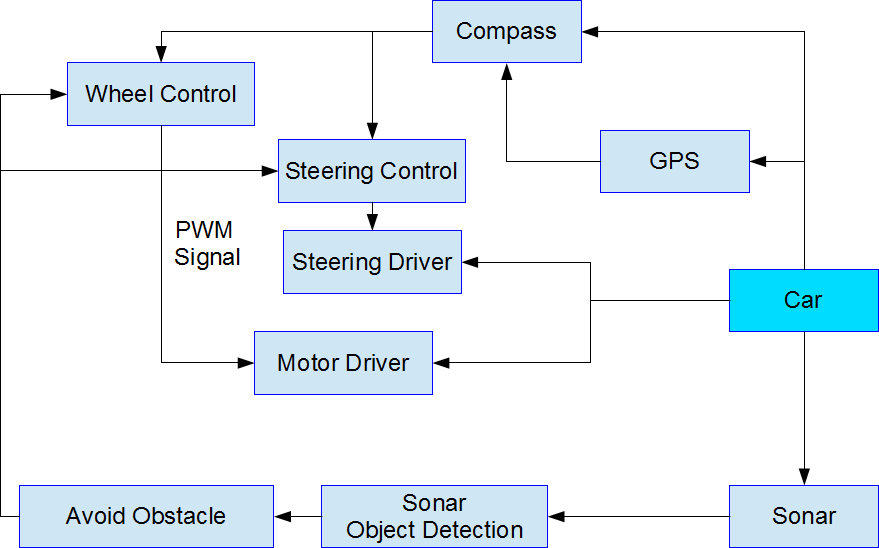
\includegraphics[scale=0.4]{HLD_A.png}
\caption{High Level Design}
\label{fig:Alg_loud}
\end{figure}
\label{sub:high_level_design}
\begin{figure}[H]
\center
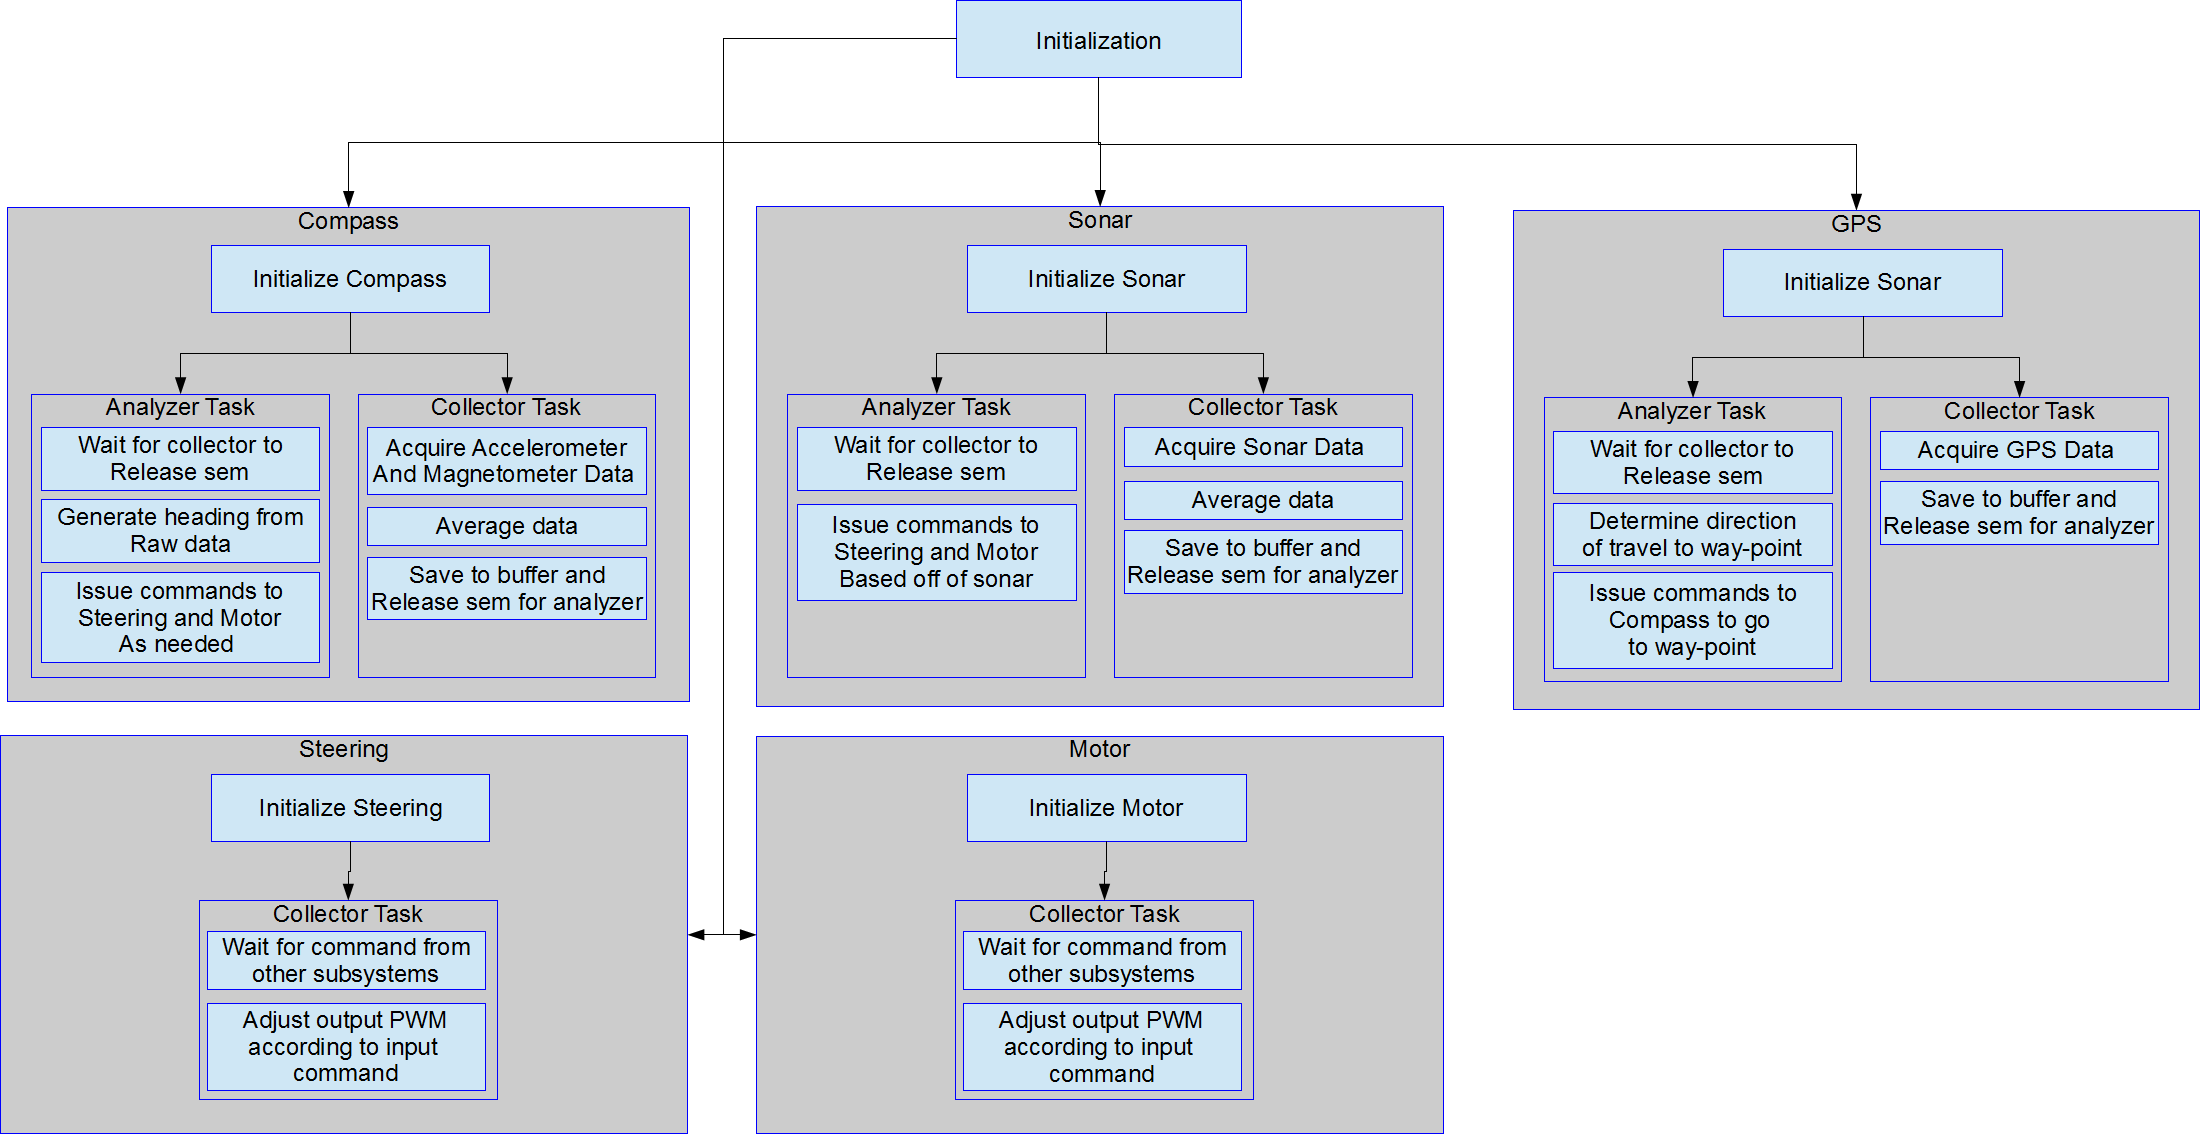
\includegraphics[scale=0.2]{HLD_B.png}
\caption{High Level Design}
\label{fig:Alg_loud}
\end{figure}
\label{sub:high_level_design}
\begin{figure}[H]
\center
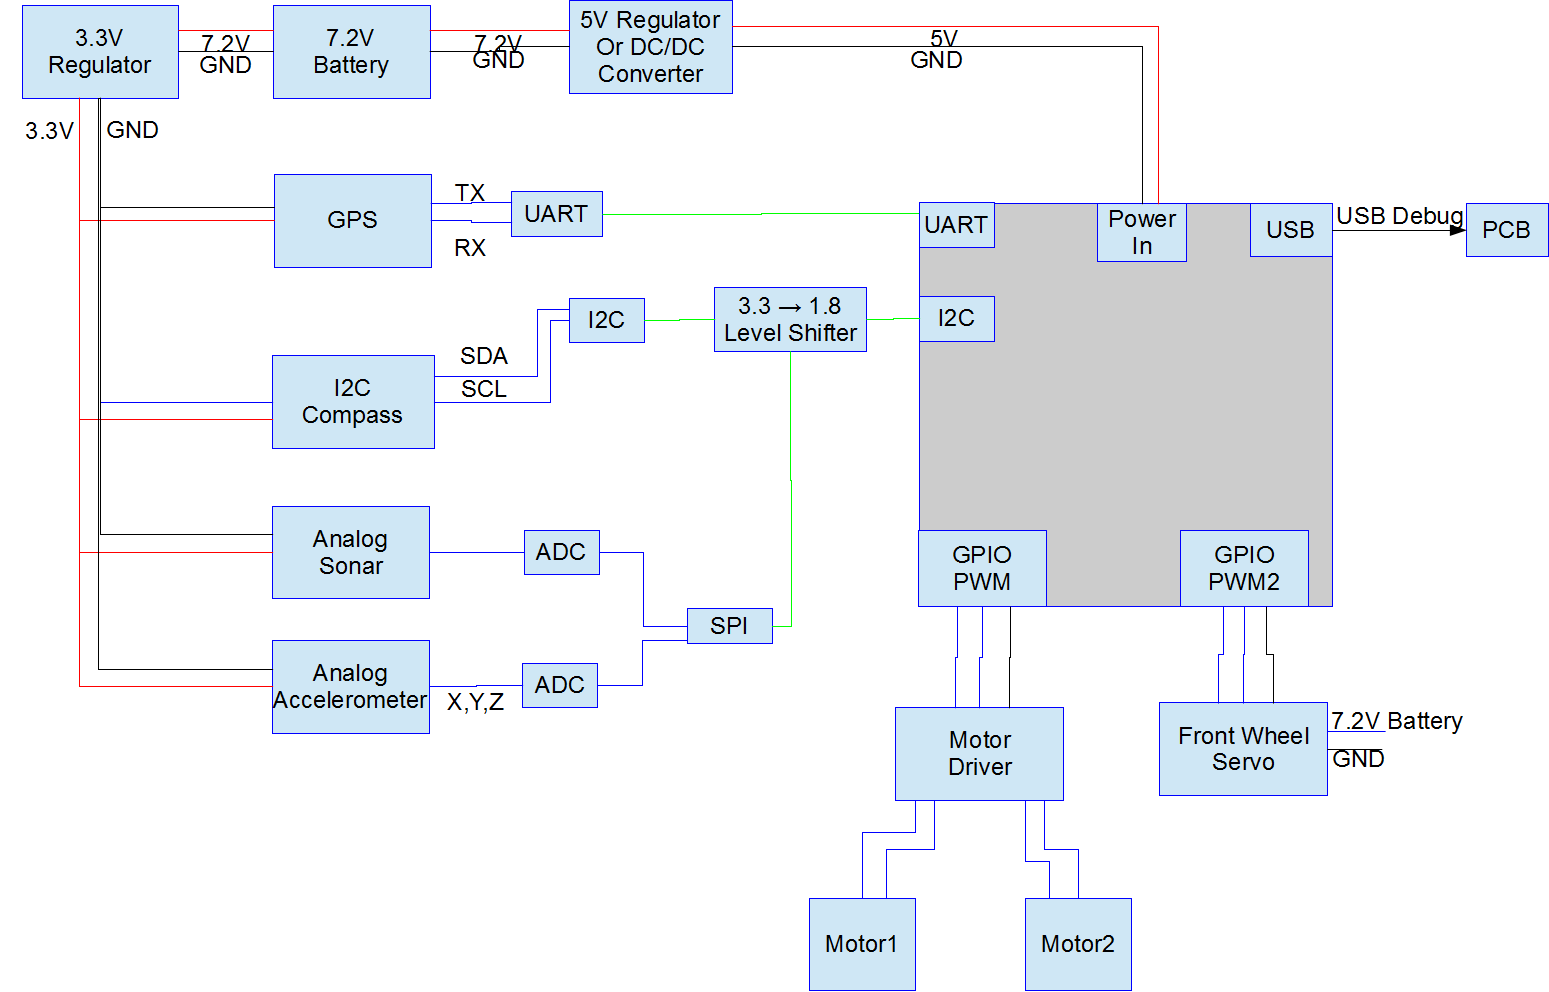
\includegraphics[scale=0.2]{HLD_C.png}
\caption{High Level Design}
\label{fig:Alg_loud}
\end{figure}
% subsection high_level_design (end)

\pagebreak

\subsubsection{Low Level Design} % (fold)
\label{ssub:low_level_design}
\begin{figure}[H]
\center
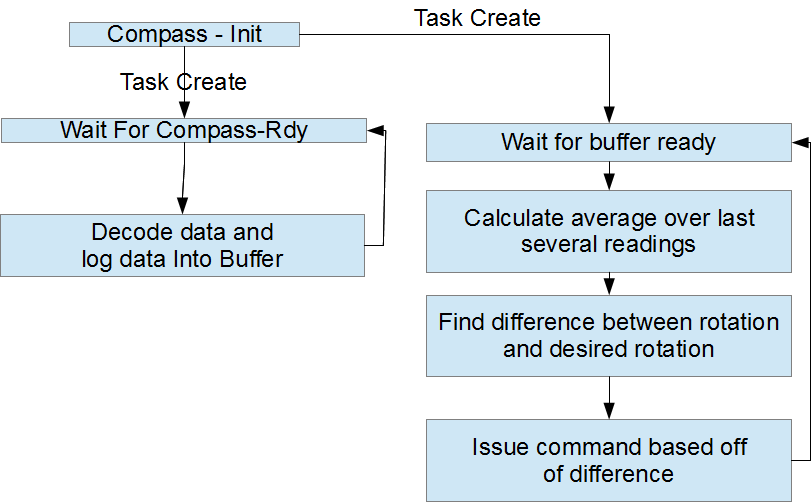
\includegraphics[scale=0.2]{LLD_Comp.png}
\caption{Low Level Compass}
\label{fig:ll_comp}
\end{figure}
\begin{figure}[H]
\center
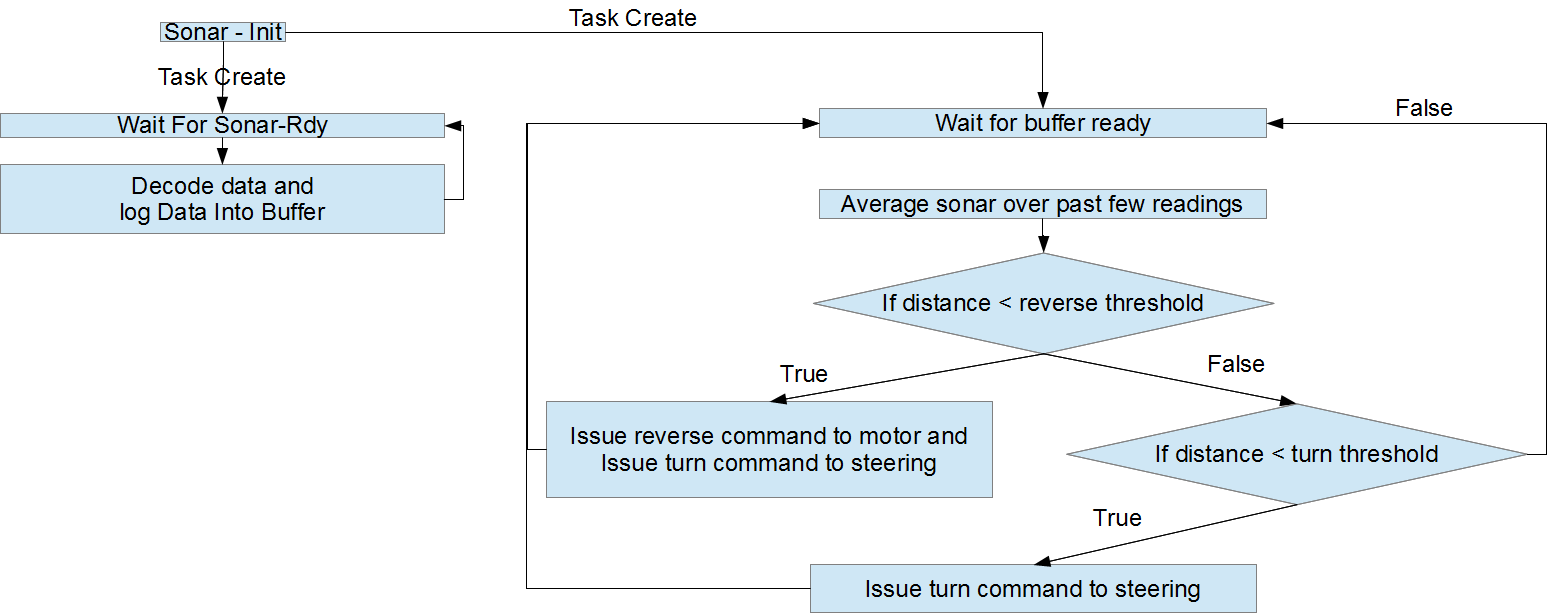
\includegraphics[scale=0.2]{LLD_Sonar.png}
\caption{Low Level Sonar}
\label{fig:ll_sonar}
\end{figure}
\begin{figure}[H]
\center
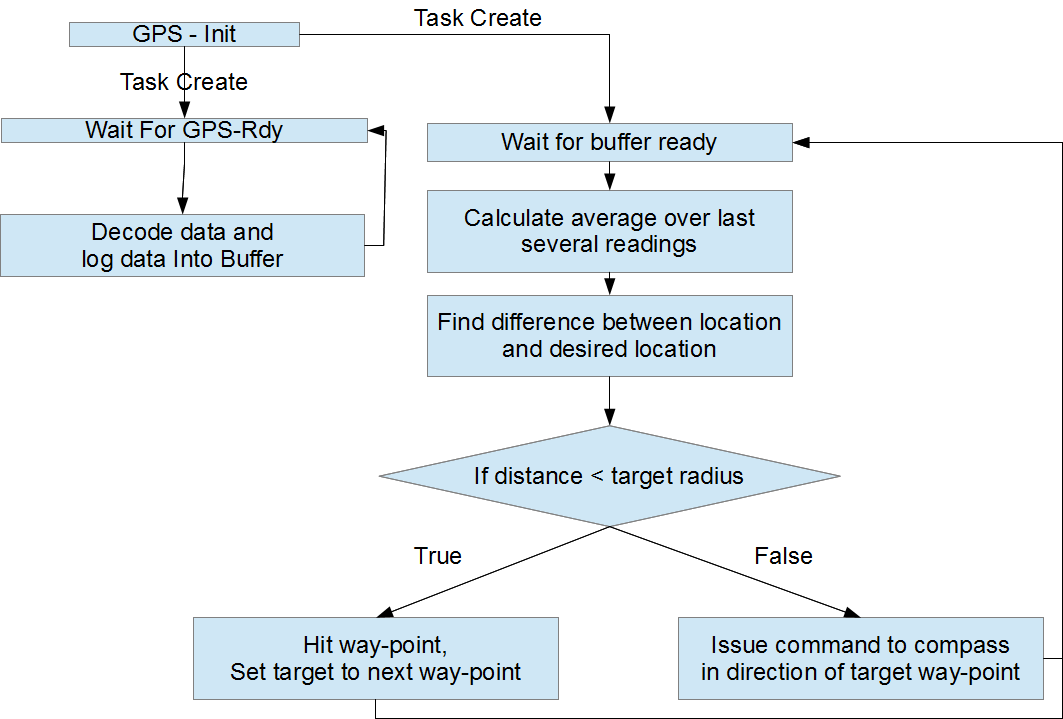
\includegraphics[scale=0.2]{LLD_GPS.png}
\caption{Low Level GPS}
\label{fig:ll_gps}
\end{figure}
% subsubsection low_level_design (end)

\pagebreak

\subsubsection{Compass} % (fold)
\label{ssub:compass}
The compass subsystem was designed to control the direction of the car when the car was not in reversal or turning mode of operation (as set by the sonar task). If the sonar was controlling the the car, the compass would not try to adjust the direction because commands from the sonar to control the car are considered more important than commands from the compass. The result is that car's primary objective is to avoid obstacles. If it is able to do that, then it will take into account commands from the compass. The compass subsystem was designed to collect data directly from both the magnetometer and the accelerometer (using the collector task). It would then use both data values to determine the direction of north with respect to the front of the car (using the analyzer task). The compass subsystem would then issue commands to the steering subsystem to point the car towards a target declination. \\
The collector task collected data from the magnetometer and the accelerometers using SPI to communicate with an external ADC. After collecting the data, the collector would average the data as necessary to reduce noise and finally store the acceleration vector $A$ and compass vector $B$ into a buffer. The analyzer task would then read from the buffer and convert the vectors $A$ and $B$ into a north vector $N$ which pointed in the direction of north in the car's coordinate system. The $N$ vector was determined by taking $\bar N=A \cdot \left(\bar B \cdot \bar G\right)$ as mentioned in the design challenges section of this report [Section~\ref{sub:magnetometer}]. The $N$ vector was then projected onto the $xy$ plane and the angle was found using the inverse tangent of the X and Y coordinates of the $N$ vector. Upon determine the angle of north from the front of the car, a small rotational offset was added to the declination in order to take into account discrepancies between magnetic north and geographic north as well as a slight skew in how the magnetometer was mounted onto the car. After a proper north angle was determined, it was compared to the target angle of the car and commands were issued to the steering subsystem to turn the car in the proper direction accordingly.
% subsubsection compass (end)

\pagebreak

\subsubsection{GPS} % (fold)
\label{ssub:gps}
The GPS subsystem was written to set the heading in the compass subsystem to the desired direction of travel based off of the car's current location as determined by the GPS and it's desired location. The desired location was an input to the program and set by sending in a linked list of way-points. The car would travel toward the first way-point until it reached a minimum distance to the way-point at which point the car would interpret the way-point as being hit and at which point the next way-point would be set as the target. The result was that the car would traverse the way-points in order and follow them like a path. The direction between the current location and the desired location was found using geometry and this angle was set as the target of the compass subsystem. This kept the GPS system simple because all it was required to do to change the direction of the car was to tell the compass subsystem what direction the car should be pointed toward.
% subsubsection gps (end)

\subsubsection{Steering} % (fold)
\label{ssub:steering}
The steering subsystem received commands from both the compass and the sonar. The commands received would determine what direction the front wheels should be pointed. Because this subsystem would only every issue commands (and never collect data), it was designed to only have one task called a mechanical controller. This task would wait for input from one of the other subsystems, then send commands to the steering servo through PWM signals. 
% subsubsection steering (end)

\subsubsection{Motor} % (fold)
\label{ssub:motor}
The motor subsystem behaved very similar to the way the steering subsystem did. The single mechanical controller task waited for commands from other subsystems then issued the proper signals to the motor through PWM.
% subsubsection motor (end)

% subsection software (end)
% section design_as_built (end)

\pagebreak

\section{Design Challenges} % (fold)
\label{sec:design_challenges}

\subsection{GPS Accuracy} % (fold)
\label{sub:gps_accuracy}
We experienced some issues with getting accurate GPS data at a fast rate. We solved the issue of slow GPS recording by adjusting the GPS settings to collect the latitude and longitude 5 times a second. Even with this rate however, a few GPS reading returned bad latitudes and longitudes. This issue was fixed by check how valid each of the GPS coordinates were. This was done by noticing that the probability of receiving a good coordinate was much higher then the probability of a bad coordinate. To implement this, we ran a check on every coordinate. If the coordinate was not within a particular distance of previously valid coordinates (approximately 0.25 miles), the coordinate was dropped because it would imply that the robot was moving much faster than it is physically capable of moving. We then took a rolling average of the valid GPS coordinates to reduce noise.
% subsection gps_accuracy (end)

\subsection{Magnetometer} % (fold)
\label{sub:magnetometer}
One of the issues faced in this project was bad compass readings. This was because initially we decided to use a single axis magnetometer as a compass which works well on flat ground, but quickly changes values on angled ground. The result was that the robot would head in the correct direction only if it was on a flat surface and would diverge from its path significantly when the surface was not flat. To fix this problem, we switched to using a triple axis magnetometer along side a triple axis accelerometer. The reason the initial approach did not work was because the robot had no information about its orientation and couldn't possibly know which direction to travel based purely off of a magnetometer vector. We initially assumed that the robot would always be on a flat surface, but it was found that this assumption was not valid as the angle of the robot change greatly as it moved around.\\
Adding the accelerometer to this system allowed the robot to have some general sense of what direction was downward. This approach assumed that the accelerations in the horizontal $xy$ plane would be much less then the acceleration due to gravity on the $z$ axis. Now that the robot had information on which direction was down along with which direction the earths magnetic field was pointing, it was possible to determine an approximate direction of north with much higher accuracy to the original approach. North was found by taking the second dot product of the acceleration and magnetization ($\bar N=A \cdot \left(\bar B \cdot \bar G\right)$). This calculation determined the north vector $\bar N$ by projecting the magnetization vector $B$ onto the plane orthogonal to the direction of gravity $G$ and situation at the origin. The result was a much more accurate compass heading that remained accurate as long as the robot remained upright (which was a valid assumption to make).
% subsection magnetometer (end)

\subsection{Steering Noise} % (fold)
\label{sub:steering_noise}
It was found that there was noise caused by the compass which resulting in the car experiencing a strange steering pattern. The noise was tracked back to two sources: the magnetometer and the accelerometer. The noise from the magnetometer was caused by an electro-magnetic field generated by the motor. We attempted to correct this problem by placing the magnetometer far away from the motors and only running the motor at a relatively slow speed so that it did not generate a large EMF. The noise in the accelerometer was present even when the accelerometers were isolated and stationary. To fix this noise, we took a rolling average of the accelerometer points which served as a low pass filter which prevented small variations in the accelerometer readings from changing the calculated north vector. Taking the average also solved the issue of noise introduced from the car accelerating in a particular direction because the car usually experienced accelerations that had a short duration but large magnitude.
% subsection steering_noise (end)
% section design_challenges (end)

\pagebreak

\section{Final Results} % (fold)
\label{sec:final_results}

% section final_results (end)
\pagebreak
\section{Future Additions} % (fold)
\label{sec:future}
Further work with this project would includes adding more sonar sensors to the car giving it a better insight of its surroundings. Doing so would help the avoidance algorithm react to certain situation more appropriately rather than just turning the wheels in an arbitrary direction. It would also improve the reversal algorithm in a way that prevents the car from backing up into another obstacle or getting stuck in a corner.\\
Another addition to the project would be adding a camera to it and enabling OpenCV which would give the car even more information about its surroundings and would allow the car to respond to particular shapes and colors in different ways. This may be useful for running around a track in which different obstacles are marked with different colors and require the car to to different things when encountered. For example in the SparkFun challenge, yellow markers indicate poles that the car should weave around and a red hoop indicates a hoop that the car must go through.
% section future (end)
\end{document}
